% Autor: Simon May
% Datum: 2017-10-05
% Diese Datei bietet ein minimalistisches Grundgerüst für ein LaTeX-Dokument,
% z.B. für die Bearbeitung der Aufgaben.
\documentclass[
	% Papierformat
	a4paper,
	% Schriftgröße (beliebige Größen mit „fontsize=Xpt“)
	12pt,
	% Schreibt die Papiergröße korrekt ins Ausgabedokument
	pagesize,
	% Sprache für z.B. Babel
	ngerman
]{scrartcl}

% Achtung: Die Reihenfolge der Pakete kann (leider) wichtig sein!
% Insbesondere sollten (so wie hier) babel, fontenc und inputenc (in dieser
% Reihenfolge) als Erstes und hyperref und cleveref (Reihenfolge auch hier
% beachten) als Letztes geladen werden!

% Silbentrennung etc.; Sprache wird durch Option bei \documentclass festgelegt
\usepackage{babel}
% Verwendung der Zeichentabelle T1 (Sonderzeichen etc.)
\usepackage[T1]{fontenc}
% Legt die Zeichenkodierung der Eingabedatei fest, z.B. UTF-8
\usepackage[utf8]{inputenc}
% Schriftart
\usepackage{lmodern}
% Zusätzliche Sonderzeichen
\usepackage{textcomp}

% Mathepaket (intlimits: Grenzen über/unter Integralzeichen)
\usepackage[intlimits]{amsmath}
% Ermöglicht die Nutzung von \SI{Zahl}{Einheit} u.a.
\usepackage{siunitx}
% Zum flexiblen Einbinden von Grafiken (\includegraphics)
\usepackage{graphicx}
% Abbildungen im Fließtext
\usepackage{wrapfig}
% Abbildungen nebeneinander (subfigure, subtable)
\usepackage{subcaption}
% Funktionen für Anführungszeichen
\usepackage{csquotes}
% Zitieren, Bibliographie
\usepackage{biblatex}

% Verlinkt Textstellen im PDF-Dokument
\usepackage[unicode]{hyperref}
% "Schlaue" Referenzen (nach hyperref laden!)
\usepackage{cleveref}

% siunitx: Deutsche Ausgabe, Messfehler getrennt mit ± ausgeben
\sisetup{
	locale=DE,
	separate-uncertainty
}

\begin{document}
\begin{titlepage}
	\centering
	{\scshape\LARGE Versuchsbericht zu \par}
	\vspace{1cm}
	{\scshape\huge E4\par}
	\vspace{2.5cm}
	{\LARGE Gruppe 2 Mo\par}
	\vspace{0.5cm}
	{\large Nils Kulawiak (E-Mail: n\_kula01@wwu.de) \par}
	{\large Oliver Brune (E-Mail: o\_brun02@wwu.de) \par}
	\vfill
	durchgeführt am 15.1.2017\par
	
	\vfill

	{\large \today\par}
\end{titlepage}


\tableofcontents
	
	
\newpage
\section{Einleitung}
In diesem Versuch werden Phasenübergänge von einer Cu$_{3}$Au Mischung unter Variation der Temperatur betrachtet. Im ersten Teil des Versuchs wird das erreicht, indem das Debye-Scherrer Verfahren angewendet wird. Dabei wird eine polykristalline Probe mit monochromatischer Röntgenstrahlung unter Variation des Drehwinkels bestrahlt.

Ziel bei dieser Untersuchung ist es die Gitterkonstante a des fcc-Gitters zu bestimmen und ihre lineare Abhängigkeit von der Temperatur zu überprüfen. Außerdem soll geschaut werden, ob die Kernaussagen die Debye mathematisch hergeleitet hat auch experimentell bestätigt werden können.
\section{Interferenz von Röntgenstrahlen unter Erhöhung der Temperatur}
\subsection{Methoden und Durchführung}

\subsection{Auswertung}
\subsubsection{Gitterkonstante}
Ziel dieses Teil des Versuches ist es die Phasenumwandlung einer Kupfer-Gold Mischung für verschiedene Temperaturen zu untersuchen, wobei bekannt ist, dass es sich um ein fcc-Gitter handelt. Das wird erreicht, indem diese Mischung unter sich verändernden Winkel mit Röntgenstrahlung bestrahlt wird und die Intensität dazu gemessen wird. Wenn es zu einer konstruktiven Interferenz kommt, kann mithilfe der Bragg-Gleichung auf den Abstand der Ebenen voneinander geschlossen werden:
\begin{equation}
2d sin(\theta) = n \lambda
\label{bragg}
\end{equation}

Wenn bekannt ist um was für eine Ebene es sich handelt, kann daraus wiederum der Gitterabstand eines kubischen Gitters berechnet werden.

\begin{equation}
d = \frac{a}{\sqrt{h^{2}+k^{2}+l^{2}}}
\label{d}
\end{equation}

Damit lässt sich daraufhin zeigen, wie sich der Gitterabstand mit der Temperatur verändert, wobei ein linearer Anstieg erwartet wird, anhand von 
\begin{equation}
<r-r_{0}> = \frac{3 b}{4 a^{2}} k_{b} \cdot T, 
\label{Temp}
\end{equation}
wobei alles außer die Temperatur T Konstanten sind.

Der Phasenübergang lässt sich mit der sogenannten Fernordnung beschreiben, welche aussagt wie geordnet ein Kristallgitter ist, wobei $\mu$ = 1 für eine vollständige Ordnung und $\mu$ = 0 für vollständige Unordnung steht. Ein fcc-Gitter lässt sich in vier verschiedene sc-Gitter aufteilen. Bei einer vollständigen Ordnung befinden sich alle Goldatome auf dem sc-Gitter mit der Basis (0,0,0), während sich die Kupferatome auf den anderen drei sc-Gitter befinden.
Bei einer vollständigen Unordnung ist es rein zufällig, wie die Gold und Kupferatome verteilt sind.

Die Intensität hängt dabei auch indirekt mit der Intensität bzw. der Fernordnung zusammen.
\begin{equation}
I_{hkl} \propto |F_{hkl}|^{2} \cdot p \cdot L_{p} \cdot D_{T}.
\end{equation}

\begin{itemize}


\item Der Flächenhäufigkeitsfaktor p beschreibt dabei wie häufig eine Ebene in der Gitterstruktur vorkommt.

\item Der Lorentz-Polarisationsfaktor $L_{p}$ korrigiert verschiedene Effekte der Röntgenbeugung und beträgt $L_{p} =\frac{1 + cos^{2}(2 \theta)}{sin^{2}(\theta) cos(\theta)}$. 

\item Der Debye-Waller-Faktor beschreibt den Einfluss der Wärmebewegung auf die Intensität und beträgt $D_{T} = \text{exp}(-2B \cdot \frac{sin^{2}(\theta)}{\lambda^{2}})$, wobei B ein experimentell bestimmter Wert ist.

\item Der Strukturfaktor $F_{hkl}$ beschreibt das Streuvermögen einer Elementarzelle.
\end{itemize}

Um den Streufaktor zu berechnen wird über alle Basisatome summiert.
\begin{equation}
F_{hkl} \propto \sum_{i=1}^{n} f_{i} e^{2 \pi i(hx_{i} + ky_{i} + lz_{i})}
\end{equation}

Da sich die Basisatome bei $(0,0,0) ; (\frac{a}{2},\frac{a}{2},0) ; (\frac{a}{2},0,\frac{a}{2})$ und $(0, \frac{a}{2}, \frac{a}{2})$ befinden, ergibt sich der Streufaktor bei vollständiger Ordnung zu 
\begin{equation}
F_{hkl} = f_{Au} + f_{Cu} (e^{2 \pi i(h+l)} + e^{2 \pi i(k+l)} + e^{2 \pi i(h+k)}).
\end{equation}

Somit ergibt sich für jede Ebene ein Peak, allerdings sind die Peaks mit nur geraden oder ungeraden h,k und l deutlich größer, da der Strukturfaktor dort $f_{Au} + 3f_{Cu}$ ergibt und sonst $f_{Au} - f_{Cu}$.

Anders verhält es sich bei der vollständigen Unordnung. Dort ergibt sich der Strukturfaktor zu 
\begin{equation}
F_{hkl} = (\frac{1}{4} f_{Au} + \frac{3}{4}f_{Cu}) (1 + e^{2 \pi i(h+l)} + e^{2 \pi i(k+l)} + e^{2 \pi i(h+k)}).
\end{equation}

Somit bleibt der Strukturfaktor gleich für alle h,k und l gerade oder ungerade, allerdings ergibt sich der Strukturfaktor für alle anderen Ebenen zu 0. 
Die Röntgenreflexe, die immer unabhängig von der Fernordnung erscheinen, nennt man Fundamentalreflex, während die sich ändernden Überstrukturreflex genannt werden.

Unter der Annahme, dass der Strukturfaktor linear mit der Fernordnung $\mu$ skaliert ergibt er sich zu
\begin{equation}
F_{hkl} = \left \{ \begin{array}{ll}
f_{Au} + 3f_{Cu} \text{  für nur gerade oder ungerade h,k,l} \\
\mu \cdot (f_{Au} - f_{Cu}) \text{  sonst} \\
\end{array} \right.
\end{equation}

Das entspricht auch den experimentellen Ergebnissen Ergebnissen. In \cref{25} sind alle möglichen Ebenen bis (3 1 1) vorhanden, während in \cref{400} nur der Fundamentalreflex zu sehen ist. Dies ändert sich auch nicht für höhere Temperaturen von 500 bzw. 700°C. 
Daraus lässt sich schließen, dass es bei der Temperaturerhöhung von 25 auf 400°C zu einem Phasenübergang gekommen ist. Am Anfang ist Die Fernordnung $\mu$ deutlich größer als null, während sie später ungefähr gleich null ist. Dies entspricht auch den bisherigen Erkenntnissen, welche einen Phasenübergang bei 390°C erwarten. Allerdings lässt sich mit dieser Methode nicht herausfinden wie groß die Fernordnung genau ist. 

Außerdem lassen sich die Gitterkonstanten mithilfe von \cref{bragg} und \cref{d} berechnen. Beispielhaft wird dies hier für \cref{400} gemacht:
\begin{table}[h]
\caption{Gitterabstand a bei 400°}
\begin{tabular}{|l|l|l|l|}
\hline
Fläche & Winkel $2 \theta${[}°{]} & Flächenabstand d {[}\AA{]} & Gitterabstand a {[}\AA{]} \\ \hline
111    & 41,62                     & 2,1674        & 3,7540      \\ \hline
200    & 48,4                      & 1,8784        & 3,7568       \\ \hline
220    & 70,64                     & 1,3319        & 3,7670       \\ \hline
331    & 85,24                     & 1,1371         & 3,7715       \\ \hline
\end{tabular}
\end{table} 

Wenn dieser Vorgang für die anderen Temperaturen wiederholt wird, ergibt sich der aus \cref{Temp} erwartete lineare Anstieg.
\begin{figure}[h]
	\centering
	\includegraphics[scale=0.35]{Lin.PNG}
	\caption{Gitterabstand in Abhängigkeit der Temperatur}
	\label{Temp}
\end{figure}

\begin{figure}[h]
	\centering
	\includegraphics[scale=0.35]{25.PNG}
	\caption{Intensitätsverteilung bei Raumtemperatur}
	\label{25}
\end{figure}


\begin{figure}[h]
	\centering
	\includegraphics[scale=0.35]{400.PNG}
	\caption{Intensitätsverteilung bei 400°C}
	\label{400}
\end{figure}

\subsubsection{Debye}

Außerdem sollen noch die Kernaussagen von Debye überprüft werden. Die erste Aussage heißt:

"Die Schärfe der Interferenzmaxima wird durch die Wärmebewegung nicht beeinflusst."


Die Breite (und damit Schärfe) der Interferenzmaxima wird bestimmt, indem die Halbwertsbreite für die Ebenen (1 1 1) und (2 0 0) als Breite angenommen werden und für die Ebenen (2 2 0) und (3 1 1)  Der Punkt auf dem sie unter $\frac{3}{4}$ ihres Höchstwerts fallen. Diese wurde gemacht, wegen der geringen Intensität der beiden hinter Fundamentalpeaks, weshalb die Hintergrundstrahlung häufig bei der Halbwertsbreite interferiert hat. Unter diesen Annahmen ergibt sich eine Schärfe der einzelnen Peaks von:
\begin{table}[h]
\caption{Schärfe der Interferenzpeaks in Grad}
\begin{tabular}{l|llll}
Temperatur[°C] \textbackslash{}Fläche & 110  & 200  & 220  & 311  \\ \hline
25                               & 0,46 & 0,4  & 0,18 & 0,14 \\
400                              & 0,34 & 0,58 & 0,1  & 0,1  \\
500                              & 0,58 & 0,74 & 0,2  & 0,2  \\
700                              & 0,64 & 0,64 & 0,16 & -   
\end{tabular}
\end{table}

In der Tabelle lässt sich zwar ein Anstieg der Breite mit der Temperatur erahnen, besonders bei den beiden Halbwertsbreiten, die deutlich genauer sind, da sie weniger stark von einzelnen Fluktuationen beeinflusst sind. Für die beiden anderen Ebenen scheint die Schärfe mehr oder weniger zufällig zu sein. Insgesamt lässt sich also sagen, dass es zwar Indizien dafür gibt, dass die Schärfe der Intensitätspeaks mit dem Temperaturanstieg sinken, allerdings lässt sich keine eindeutige Aussage treffen. 

Die zweite Aussage von Debye sagt aus, dass sich die räumliche Intensitätsverteilung mit der Wärmebewegung ändert.

Das ist auch deutlich zu sehen, wenn die verschiedenen Fundamentalpeaks verglichen werden:
\begin{table}[h]
\caption{Position der Interferenzpeaks in Grad}
\begin{tabular}{l|llll}
Temperatur[°C] \textbackslash{}Fläche & 110   & 200   & 220   & 311   \\ \hline
25                               & 41,94 & 48,68 & 71,32 & 86,24 \\
400                              & 41,62 & 48,4  & 70,64 & 85,24 \\
500                              & 41,44 & 48,22 & 70,3  & 85,02 \\
700                              & 41,2  & 48,04 & 70,08 &      
\end{tabular}
\end{table}

Mit steigender Temperatur wird der Abstand zwischen Beobachtungs- und Einfallsebene immer kleiner. Es wurden allerdings zu wenige Messwerte aufgenommen, um festzustellen in welcher Abhängigkeit die beiden Variablen zueinander stehen.

Die letzte Aussage von Debye sagt aus, dass aufgrund der Wärmebewegung die Interferenzintensität exponentiell abnimmt
\begin{itemize}
\item mit zunehmender Temperatur 
\item mit zunehmendem Winkelabstand zwischen Einfalls- und Beobachtungsrichtung 
\item mit abnehmender Wellenlänge
\end{itemize}

Die erste Aussage spiegelt sich nicht in den experimentellen Ergebnissen wieder:
\begin{table}[h]
\caption{Intensität in kg$\cdot \text{s}^{-3}$}
\begin{tabular}{l|llll}
Temperatur[°C] \textbackslash{}Fläche & 110 & 200 & 220 & 311 \\ \hline
25                               & 165 & 151 & 96  & 109 \\
400                              & 198 & 211 & 136 & 124 \\
500                              & 251 & 154 & 124 & 182 \\
700                              & 194 & 162 & 114 &    
\end{tabular}
\end{table}

Die Intensität steigt sogar grundsätzlich beim Übergang von 25 auf 400°C. Ein exponentieller Abfall bei Zunahme der Temperatur kann also ausgeschlossen werden.

Die zweite Aussage von Debye ist zumindest nicht allgemeingültig richtig. Zwar scheint es die Intensitätsverteilung in \cref{400} gut zu beschrieben, allerdings wird offensichtlich bei Betrachtung von \cref{500}, dass sie nicht immer stimmen kann. 

Da die Wellenlänge in diesem Versuch konstant gehalten wurde, kann der letzte Punkt nicht diskutiert werden.

\begin{figure}[h]
	\centering
	\includegraphics[scale=0.3]{500.PNG}
	\caption{Intensitätsverteilung bei 500°C}
	\label{500}
\end{figure}

\begin{figure}[h]
	\centering
	\includegraphics[scale=0.3]{700.PNG}
	\caption{Intensitätsverteilung bei 700°C}
	\label{700}
\end{figure}

\section{Kalorimetrie}
\subsection{Methoden und Durchführung}
Zur Analyse des Phasenübergangs in der CuAu-Legierung wird eine kalorimetrische Untersuchung durchgeführt. Hierfür wird ein dynamisches Wärmestromdifferenzkalorimeter verwendet. Mit diesem werden Temperaturdifferenzen zwischen einer Probe und einer Referenz gemessen, die sich beide in einem Aluminiumtiegel befinden. Die Differenz ist in diesem Versuch einfach ein leerer Tiegel (Luftreferenz). Beide befinden sich dabei in einer Kammer, in der sie symmetrisch auf einer Scheibe positioniert werden ("disk-type"). Wenn die Kammer nun aufgeheizt wird, kann über die Scheibe die Temperaturdifferenz zwischen den beiden Proben ermittelt werden.

In diesem Versuch wird die Methode verwendet um den Phasenübergang zwischen Ordnung und Unordnung in der CuAu-Legierung zu untersuchen. Hierfür wird die Kammer zuerst auf eine Temperatur von $\SI{500}{\degreeCelsius}$ gebracht. Diese liegt deutlich über der Phasenübergangstemperatur, deswegen ist der Kristall in diesem Zustand ungeordnet. Anschließend wird die Kammer wieder abgekühlt, zuerst auf $\SI{410}{\degreeCelsius}$ mit einer Rate von $\SI{60}{\degreeCelsius/\minute}$, anschließend sehr langsam mit einer Rate von $\SI{5}{\degreeCelsius/\minute}$ auf $\SI{385}{\degreeCelsius}$. Diese Temperatur liegt knapp unter der Phasenübergangstemperatur von $\SI{390}{\degreeCelsius}$, daher ist nun der Phasenübergang der Legierung zu erwarten. Um diesen zu beobachten, wird die Temperatur nun für $\SI{30}{\minute}$ konstant gehalten. Der Phasenübergang von Unordnung zu Ordnung ist ein exothermer Vorgang, das heißt die Probe gibt dabei Wärme ab. Dieser Wärmefluss kann über die Temperaturdifferenz bestimmt werden. Da der Wärmefluss ein Maß für die Änderung des umgewandelten Volumens im isothermen Phasenübergang ist, kann mit diesem untersucht werden, inwiefern die Versuchsergebnisse mit der Johnson-Mehl-Avrami-Kolmogorow-Gleichung übereinstimmen.

\subsection{Auswertung}
\begin{figure}[h]
	\centering
	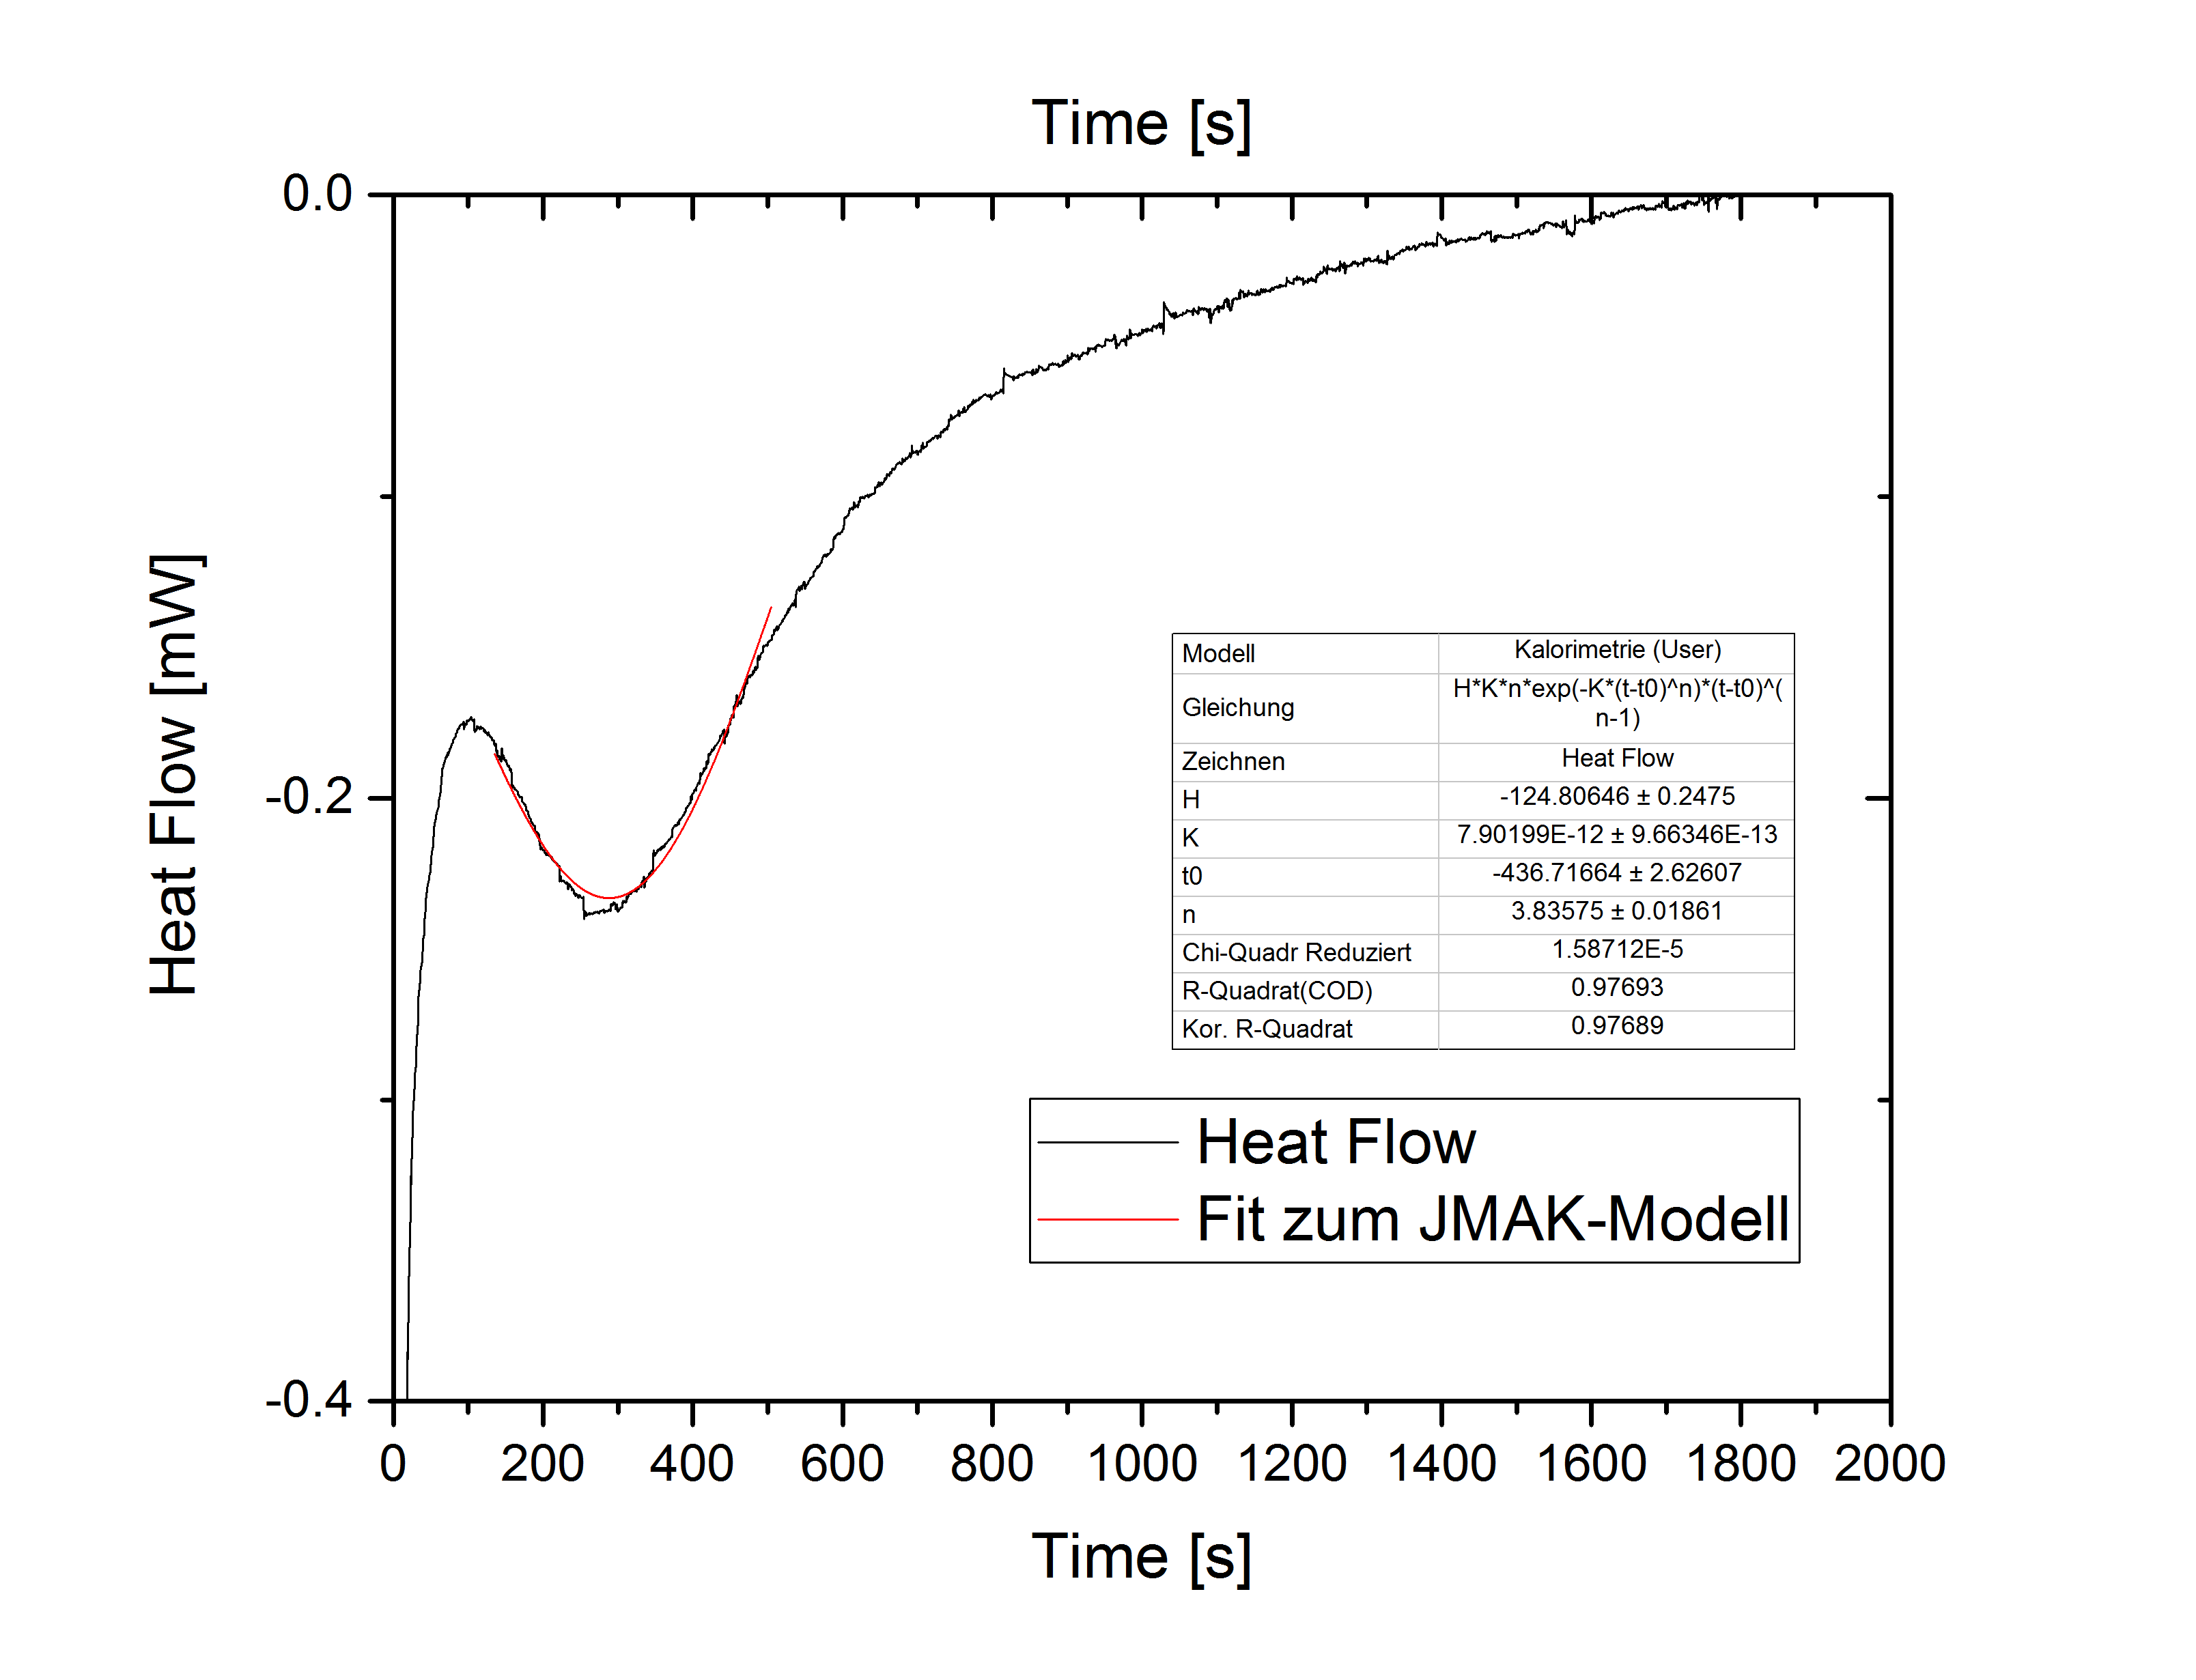
\includegraphics[scale=0.6]{Graph3.png}
	\caption{}
	\label{3}
\end{figure}	

\end{document}
